\chapter{曲线运动 万有引力与航天}
\section{曲线运动 运动的合成与分解}


1.曲线运动

(1)速度的方向

质点在某一点的速度方向,沿曲线在这一点的\_\_切线方向\_\_.

(2)运动的性质

做曲线运动的物体,速度的\_方向\_时刻在改变,所以曲线运动是\_变速\_运动.

(3)曲线运动的条件

物体所受合外力的方向跟它的速度方向\_\_不在同一条直线上\_\_或它的加速度方向与速度方向不在同一条直线上.

(4)合力方向与轨迹的关系

物体做曲线运动的轨迹一定夹在合力方向和速度方向之间,速度方向与轨迹相切,合力方向\_\_指向曲线的``凹''侧\_\_.

(5)运动类型的判断

\ding{172}判断物体是否做匀变速运动,要分析合外力是否为恒力.

\ding{173}判断物体是否做曲线运动,要分析合外力是否与速度成一定夹角.

\ding{174}匀变速曲线运动的条件:$F_{\text{合}}\neq 0$,为恒力且与速度不共线.

\ding{175}非匀变速曲线运动的条件:$F_{\text{合}}\neq 0$,为变力且与速度不共线.

2.运动的合成与分解

(1)基本概念

分运动$\dfrac{\text{运动的合成}}{\text{运动的分解}}$合运动.

(2)分解原则

根据运动的\_\_实际效果\_\_分解,也可采用正交分解.

(3)遵循的规律

位移、速度、加速度都是矢量,故它们的合成与分解都遵循\_\_平行四边形定则\_\_.

\ding{172}如果各分运动在同一直线上,需选取正方向,与正方向同向的量取``+''号,与正方向反向的量取``-''号,从而将矢量运算简化为\_\_代数运算\_\_.

\ding{173}两分运动不在同一直线上时,按照平行四边形定则进行合成,如图所示.

\ding{174}两个分运动垂直时的合成,(其大小)满足:

\begin{center}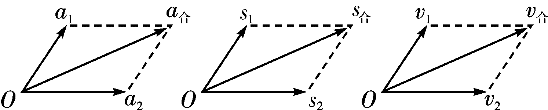
\includegraphics[width=2.48958in,height=0.5in]{media/image140.png}
	
\end{center}
$a_{\text{合}}=\sqrt{a^2_x+a^2_y}$ $s_{\text{合}}=\sqrt{x^2+y^2}$ $v_{\text{合}}=\sqrt{v^2_x+v^2_y}$

\newpage
\subsection{曲线运动的条件及特点}

{[}例1{]}(多选)质量为m的物体,在$F_1$、$F_2$、$F_3$三个共点力的作用下做匀速直线运动,保持$F_1$、$F_2$不变,仅将$F_3$的方向改变$90^\circ$(大小不变)后,物体可能做( BC )

A.加速度大小为$\dfrac{F_3}{m}$的匀变速直线运动

B.加速度大小为$\dfrac{\sqrt{2}F_3}{m}$的匀变速直线运动

C.加速度大小为$\dfrac{\sqrt{2}F_3}{m}$的匀变速曲线运动

D.匀速直线运动
\begin{solution}
	物体在$F_1$、$F_2$、$F_3$三个共点力作用下做匀速直线运动,必有$F_3$与$F_1$、$F_2$的合力等大反向,当$F_3$大小不变,方向改变$90^\circ$时,$F_1$、$F_2$的合力大小仍为$F_3$,方向与改变方向后的$F_3$夹角为$90^\circ$,故$F_{\text{合}}$=$F_3$,加速度$a=\dfrac{F_{\text{合}}}{m}=\dfrac{\sqrt{2}F_3}{m}$.若初速度方向与$F_{\text{合}}$方向共线,则物体做匀变速直线运动;若初速度方向与$F_{\text{合}}$方向不共线,则物体做匀变速曲线运动,综上所述选项B、C正确.
\end{solution}


\begin{center}
\includegraphics[width=0.70833in,height=0.125in]{media/image13.png}\end{center}

(1)判断物体是做曲线运动还是做直线运动,关键要看a和v的方向,两者方向在同一直线上则做直线运动,否则做曲线运动.

(2)曲线上某点处合外力的方向在曲线上该点的切线的哪一侧,曲线就向哪一侧弯曲;曲线轨迹必定夹在a、v方向之间.

(3)合力方向与速率变化的关系

\begin{center}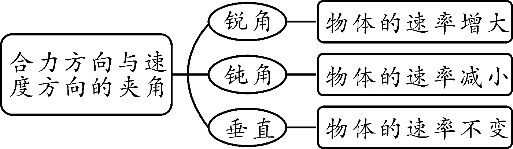
\includegraphics[width=2.33333in,height=0.67708in]{media/image142.png}\end{center}
\newpage
\subsection{运动的合成与分解}

1.运动的合成与分解的运算法则:平行四边形定则.

2.两个直线运动的合运动性质的判断标准:看合初速度方向与合加速度方向是否共线

\begin{longtable}[]{@{}ll@{}}
\toprule
两个互成角度的分运动 & 合运动的性质\tabularnewline
\midrule
\endhead
两个匀速直线运动 & 匀速直线运动\tabularnewline
一个匀速直线运动、一个匀变速直线运动 & 匀变速曲线运动\tabularnewline
两个初速度为零的匀加速直线运动 & 匀加速直线运动\tabularnewline
\multirow{2}{6cm}{两个初速度不为零的匀变速直线运动}
 &
如果$\mathrm v_{\text{合}}$与$\mathrm a_{\text{合}}$共线,为匀变速直线运动\tabularnewline
& 如果$\mathrm v_{\text{合}}$与$\mathrm a_{\text{合}}$不共线,为匀变速曲线运动\tabularnewline
\bottomrule
\end{longtable}

{[}例2{]}如图所示,在一次抗洪救灾工作中,一架离水面高为h,沿水平直线飞行的直升机A,用悬索(重力可忽略不计)救护困在湖水中的伤员B,在直升机A和伤员B以相同的水平速率匀速运动的同时,悬索将伤员吊起.设经t时间后,A、B之间的距离为l,且$l=h-2t^2$.在这段时间内关于伤员B的受力情况和运动轨迹正确的是图中的( A )

\begin{center}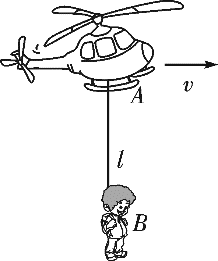
\includegraphics[width=0.98958in,height=1.1875in]{media/image143.png}\end{center}
\begin{center}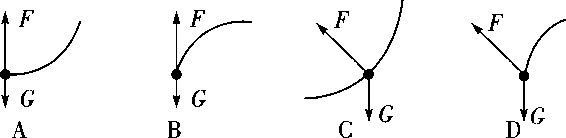
\includegraphics[width=2.57292in,height=0.625in]{media/image144.png}\end{center}
{[}思维导引{]}\ding{172}确定伤员B在水平方向和竖直方向的运动性质.\ding{173}判断伤员的运动轨迹是直线还是曲线及轨迹弯曲方向.
\begin{solution}
	由$l=h-2t^2$可知B在竖直方向为匀加速直线运动,悬索拉力大于重力,在水平方向为匀速直线运动,故运动轨迹为曲线,且向上弯曲,选项A正确.
\end{solution}


\begin{center}
\includegraphics[width=0.70833in,height=0.125in]{media/image13.png}

\textbf{合运动和分运动的关系}
\end{center}


(1)等时性:各个分运动与合运动总是同时开始,同时结束,经历时间相等(不同时的运动不能合成).

(2)独立性:一个物体同时参与几个分运动时,各分运动独立进行,互不影响.

(3)等效性:各分运动叠加起来与合运动有完全相同的效果.

(4)同一性:各分运动与合运动是指同一物体参与的分运动和实际发生的运动,不能是几个不同物体发生的不同运动.


\newpage
\subsection{小船渡河模型}

1.船的实际运动:是水流的运动和船相对静水的运动的合运动.

2.三种速度:船在静水中的速度$\mathrm v_{\text{船}}$、水的流速$\mathrm v_{\text{水}}$、船的实际速度v.

3.三种情况

\begin{longtable}[]{@{}m{0.8cm}m{2.5cm}m{10cm}@{}}
\toprule
情况 & 图示 & 说明\tabularnewline
\midrule
\endhead

渡河

时间最短
&
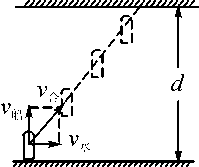
\includegraphics[width=0.90625in,height=0.76042in]{media/image146.png}
&
当船头垂直河岸时,渡河时间最短,最短时间$t_{min}=\dfrac{d}{v_{\text{船}}}$
\tabularnewline
\multirow{2}{0.8cm}{渡河位移最短}
&
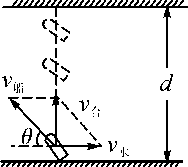
\includegraphics[width=0.85417in,height=0.76042in]{media/image147.png}
&
当$v_{\text{水}}$\textless $v_{\text{船}}$时,如果满足$v_{\text{水}}$=$v_{\text{船}}\cos
\theta$,渡河位移最短,$x_{min}=d$,此时渡河时间$t=\dfrac{d}{v_{\text{合}}}=\dfrac{d}{v_{\text{船}}}$
\tabularnewline
&
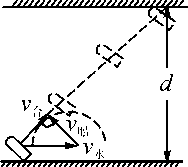
\includegraphics[width=0.85417in,height=0.76042in]{media/image148.png}
&
当$v_{\text{水}}$\textgreater $v_{\text{船}}$时,如果船头方向(即$v_{\text{船}}$方向)与合速度方向垂直,渡河位移最短,最短渡河位移为$x_{min}=\dfrac{dv_{\text{水}}}{v_{\text{船}}}$\tabularnewline
\bottomrule
\end{longtable}

{[}例4{]}(2018·湖北宜昌检测)如图所示,一艘轮船正在以4m/s的速度沿垂直于河岸方向匀速渡河,河中各处水流速度都相同,其大小为$v_1=3m/s$,行驶中,轮船发动机的牵引力与船头朝向的方向相同.某时刻发动机突然熄火,轮船牵引力随之消失,轮船相对于水的速度逐渐减小,但船头方向始终未发生变化.求:

\begin{center}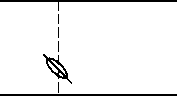
\includegraphics[width=0.80208in,height=0.4375in]{media/image149.png}\end{center}

(1)发动机未熄灭时,轮船相对于静水行驶的速度大小;

(2)发动机熄火后,轮船相对于河岸速度的最小值.
\begin{solution}(1)5 m/s (2)2.4 m/s

	(1)发动机未熄火时,轮船运动速度$v$与水流速度$v_1$方向垂直,如图所示,故此时船相对于静水的速度$v_2$的大小$v_2=\sqrt{v^2+v_1^2}=\sqrt{4^2+3^2} m/s=5 m/s$,设$v$与$v_2$的夹角为$\theta$,则$\cos \theta=\dfrac{v}{v_2} =0.8$.
\begin{center}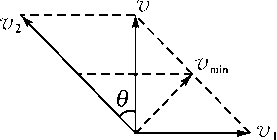
\includegraphics[width=1.26042in,height=0.63542in]{media/image150.png}\end{center}

(2)熄火前,船的牵引力沿$v_2$的方向,水的阻力与$v_2$的方向相反,熄火后,牵引力消失,在阻力作用下,$v_2$逐渐减小,但其方向不变,当$v_2$与$v_1$的矢量和与$v_2$垂直时,轮船的合速度最小,则$v_{min}=v_1\cos\theta=3\times 0.8 m/s=2.4 m/s$.
\end{solution}


\newpage
\subsection{关联速度问题}

1.模型特点

绳(杆)拉物体或物体拉绳(杆),以及两物体通过绳(杆)相连,物体运动方向与绳(杆)不在一条直线上,求解运动过程中它们的速度关系,都属于该模型.

2.模型分析

(1)合速度$\rightarrow$物体的实际运动速度v;

(2)分速度其一:沿绳或杆的速度$\mathrm v_1$;其二:与绳或杆垂直的分速度$\mathrm v_2$.

3.解题方法

把物体的实际速度分解为垂直于绳(杆)和平行于绳(杆)两个分量,根据沿绳(杆)方向的分速度大小相等求解.

4.常见模型示例

\begin{center}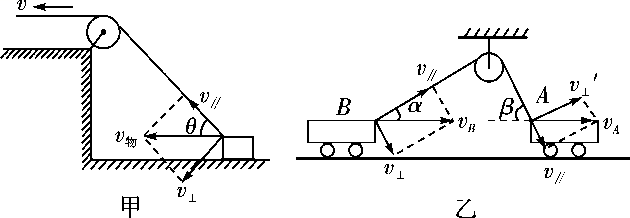
\includegraphics[width=2.86458in,height=0.98958in]{media/image151.png}\end{center}
\begin{center}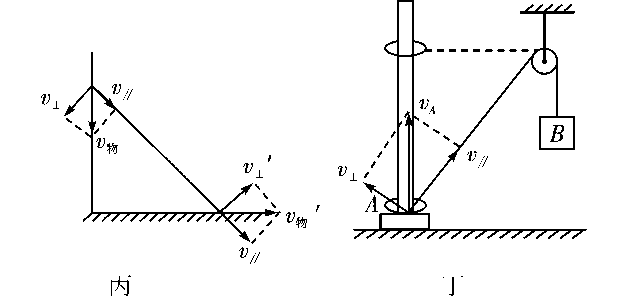
\includegraphics[width=2.85417in,height=1.35417in]{media/image152.png}\end{center}
\begin{center}
\includegraphics[width=0.70833in,height=0.125in]{media/image37.png}

\textbf{绳(杆)端速度分解的技巧}
\end{center}


(1)明确分解谁------分解不沿绳(杆)方向运动物体的速度;

(2)知道如何分解------沿绳(杆)方向和垂直绳(杆)方向分解;

(3)求解依据------因为绳(杆)不能伸长,所以沿绳(杆)方向的速度分量大小相等.

{[}例5{]}(2018·河南中原名校联考)如图所示,细线一端固定在天花板上的O点,另一端穿过一张CD光盘的中央小孔后拴着一个橡胶球,橡胶球静止时,竖直悬线刚好挨着水平桌面的边沿.现将CD光盘按在桌面上,并沿桌面边缘以速度v匀速移动,移动过程中,CD光盘中央小孔始终紧挨桌面边线,当悬线与竖直方向的夹角为$\theta$时,小球上升的速度大小为( A )

\begin{center}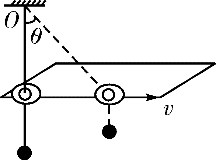
\includegraphics[width=0.97917in,height=0.72917in]{media/image153.png}\end{center}

A.vsin $\theta$ 

B.vcos $\theta$

C.vtan $\theta$ 

D.vcot $\theta$

{[}思维导引{]}光盘向右的速度是合速度.


\newpage
\section{抛体运动的规律及应用}


1.平抛运动

(1)定义:将物体以一定的初速度沿\_\_水平方向\_\_抛出,物体只在\_\_重力\_\_作用下的运动.

(2)性质:平抛运动是加速度为g的\_\_匀变速曲线\_\_运动,运动轨迹是\_\_抛物线\_\_.

(3)研究方法:运动的合成与分解.

\ding{172}水平方向:\_\_匀速直线\_\_运动;\ding{173}竖直方向:\_\_自由落体\_\_运动.

2.斜抛运动

(1)定义:将物体以初速度$v_0$\_\_斜向上方\_\_或\_\_斜向下方\_\_抛出,物体只在\_\_重力\_\_作用下的运动.

(2)性质:斜抛运动是加速度为g的\_\_匀变速曲线\_\_运动,运动轨迹是\_\_抛物线\_\_.

(3)研究方法:运动的合成与分解.

\ding{172}水平方向:\_\_匀速直线\_\_运动;\ding{173}竖直方向:\_\_匀变速直线\_\_运动.

(4)基本规律(以斜上抛运动为例,如图所示)

\begin{center}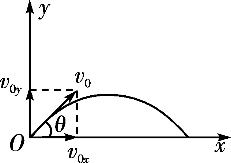
\includegraphics[width=1.05208in,height=0.73958in]{media/image160.png}\end{center}

\ding{172}水平方向:$v_{0x}=v_0\cos\theta$,$F_{\text{合}x}=0$;

\ding{173}竖直方向:$v_{0y}=v_0\sin\theta$,$F_{\text{合}y}=mg$.

\newpage
\subsection{平抛运动的基本规律}

1.关于平抛运动必须掌握的四个物理量

\begin{longtable}[]{@{}m{2cm}m{10cm}@{}}
\toprule
物理量 & 相关分析\tabularnewline
\midrule
\endhead
飞行时间(t) 
&
$t=\sqrt{\dfrac{2h}{g}}$,飞行时间取决于下落高度h,与初速度$v_0$无关\tabularnewline
水平射程(x) 
&
$x=v_0t=v_0\dfrac{2h}{g}$,即水平射程由初速度$v_0$和下落高度h共同决定,与其他因素无关\tabularnewline
落地速度(v) 
& $v=\sqrt{v_x^2+v_y^2}=\sqrt{v_0^2+2gh}$,以$\theta$表示落地时速度与x轴正方向间的夹角,有$\tan\theta=\dfrac{v_y}{v_x} =\dfrac{\sqrt{2gh}}{v_0} $,所以落地速度也只与初速度$v_0$和下落高度h有关\tabularnewline

速度的

改变量($\Delta v$)
& \begin{minipage}[t]{0.7\columnwidth}\raggedright
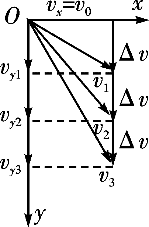
\includegraphics[width=0.67708in,height=1.03125in]{media/image161.png}

因为平抛运动的加速度为恒定的重力加速度g,所以做平抛运动的物体在任意相等时间间隔$\Delta$t内的速度改变量$\Delta$v=g$\Delta$t相同,方向恒为竖直向下,如图所示\strut
\end{minipage}\tabularnewline
\bottomrule
\end{longtable}

2.平抛运动的两个重要推论

\begin{center}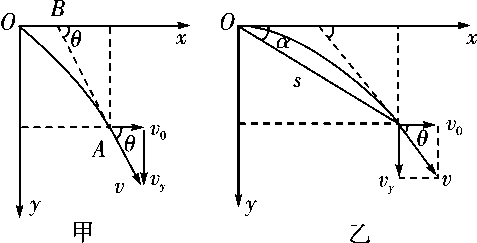
\includegraphics[width=2.16667in,height=1.10417in]{media/image162.png}
	
\end{center}

(1)做平抛运动的物体任一时刻的瞬时速度的反向延长线一定通过此时水平位移的中点,如图甲中A点和B点所示.其推导过程为$\tan \theta=\dfrac{v_{y}}{v_{x}}=\dfrac{g t^{2}}{v_{0} t}=\dfrac{y}{\dfrac{x}{2}}$.

(2)做平抛运动的物体在任一时刻任一位置处,设其速度方向与水平方向的夹角为$\theta$,位移与水平方向的夹角为$\alpha$,则tan
$\theta=2\tan \alpha$.如图乙所示.其推导过程为$\tan\theta=\dfrac{v_{y}}{v_{0}}=\dfrac{g t \cdot t}{v_{0} \cdot t}=\dfrac{2 y}{x}=2 \tan \alpha$.

\begin{center}
\includegraphics[width=0.70833in,height=0.125in]{media/image37.png}

\textbf{``化曲为直''思想在平抛运动中的应用}
\end{center}


根据运动效果的等效性,利用运动分解的方法,将其转化为我们所熟悉的两个方向上的直线运动:

(1)水平方向的匀速直线运动;

(2)竖直方向的自由落体运动.

\newpage
\subsection{与斜面关联的平抛运动}

\begin{longtable}[]{@{}m{2cm}m{3cm}m{3cm}m{5cm}@{}}
\toprule
方法 & 运动情景 & 定量关系 & 总结\tabularnewline
\midrule
\endhead
\multirow{2}{2cm}{分解速度}
&
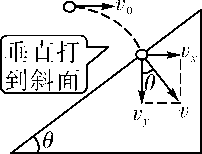
\includegraphics[width=0.91667in,height=0.69792in]{media/image163.png}
&
$v_x=v_0$

$v_y=gt$

$\tan \theta=\dfrac{v_{x}}{v_{y}}=\dfrac{v_{0}}{g t}$
&
\multirow{2}{5cm}{速度方向与$\theta$有关,分解速度,构建速度三角形}

\tabularnewline
& 
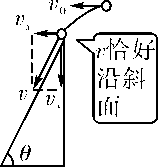
\includegraphics[width=0.71875in,height=0.76042in]{media/image164.png}
&
$v_x=v_0$

$v_y=gt$

$\tan \theta=\dfrac{v_{x}}{v_{y}}=\dfrac{g t}{v_{0}}$

& \tabularnewline
\multirow{2}{2cm}{分解位移}
& 
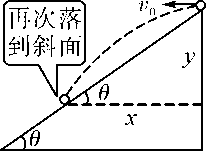
\includegraphics[width=0.9375in,height=0.6875in]{media/image165.png}
&
$x=v_0t$

$y=\dfrac{1}{2} gt^2$

$\tan \theta=_{x}^{y}=\dfrac{g t}{2 v_{0}}$
& 
\multirow{2}{5cm}{位移方向与$\theta$有关,分解位移,构建位移三角形}
\tabularnewline
&
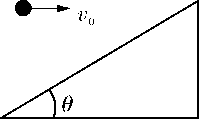
\includegraphics[width=0.90625in,height=0.54167in]{media/image166.png}

到达斜面位移最小
&
$x=v_0t$

$y=\dfrac{1}{2} gt^2$

$\tan \theta=_{x}^{y}=\dfrac{2 v_{0}}{g t}$
 & \tabularnewline
\bottomrule
\end{longtable}

{[}例2{]}(2018·湖北黄冈调研)如图所示,小球以$v_0=10m/s$的速度水平抛出,斜面的夹角$\theta=37^\circ$,取 $g=10m/s^2$,$\sin 37^\circ=0.6$,$\cos37^\circ=0.8$,不计空气阻力.

(1)若小球垂直打到斜面上,求飞行时间$t_1$;

(2)若小球到达斜面的位移最小,求飞行时间$t_2$.

\begin{center}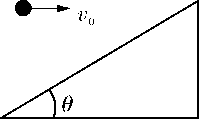
\includegraphics[width=0.90625in,height=0.54167in]{media/image166.png}\end{center}
\begin{solution}
	(1) $\dfrac{4}{3}s$ (2) $\dfrac{8}{3}s$
\end{solution}
\newpage
\subsection{平抛运动中的临界问题}

\begin{center}
\includegraphics[width=0.70833in,height=0.125in]{media/image37.png}\end{center}

(1)处理平抛运动中的临界问题应抓住两点

\ding{172}找出临界状态对应的临界条件;

\ding{173}要用分解速度或者分解位移的思想分析平抛运动的临界问题.

(2)平抛运动临界问题的分析方法

\ding{172}确定运动性质;

\ding{173}确定临界状态;

\ding{174}确定临界状态的运动轨迹,并画出轨迹示意图.

{[}例3{]}(2018·陕西西安调研)如图所示,水平屋顶高H=5 m,围墙高h=3.2
m,围墙到房子的水平距离L=3 m,围墙外空地宽x=10
m,为使小球从屋顶水平飞出落在围墙外的空地上,g取10 $m/s^2$.求:

\begin{center}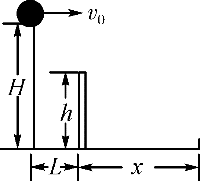
\includegraphics[width=0.90625in,height=0.82292in]{media/image169.png}\end{center}

(1)小球离开屋顶时的速度$v_0$的大小范围;

(2)小球落在空地上的最小速度的大小.

{[}思维导引{]}
(1)求出小球恰好落到空地边缘时水平初速度$v_{01}$和小球恰好越过墙的边缘的水平初速度$v_{02}$.(2)明确小球落在空地上的最小速度对应的水平初速度.
\begin{solution}(1)$5 m/s\leq v_0\leq 13 m/s$ (2)5 m/s

	(1)设小球恰好落到空地的右侧边缘时的水平初速度为$v_{01}$,则小球的水平位移$L+x=v_{01}t_1$,

小球的竖直位移$H=\dfrac{1}{2} g t^{2}$,

解以上两式得$v_{01}=(L+x) \sqrt{\dfrac{g}{2 H}}=13 \mathrm{m} / \mathrm{s}$.

设小球恰好越过围墙的边缘时的水平初速度为$v_{02}$,则此过程中小球的水平位移$L=v_{02}t_2$,

小球的竖直位移$H-h=\dfrac{1}{2} g t_{2}$,

解以上两式得$v_{02}=5 m/s$,

小球抛出时的速度大小的范围为 $5 m/s\leq v_0\leq 13 m/s$.

(2)小球落在空地上,下落高度一定,落地时的竖直分速度一定,当小球恰好越过围墙的边缘落在空地上时,落地速度最小.

竖直方向$v_{y}^{2}=2 g H$,

又有$v_{\min }=\sqrt{v_{02}^{2}+v_{y}^{2}}$,

解得$v_{\min }=5 \sqrt{5} \mathrm{m} / \mathrm{s}$.


\end{solution}

\newpage
\subsection{类平抛运动}

\begin{center}
\includegraphics[width=0.70833in,height=0.125in]{media/image37.png}\end{center}

(1)类平抛运动与平抛运动的处理方法相同,但要搞清楚其加速度的大小和方向.

(2)需注意的是,类平抛运动的初速度的方向不一定是水平方向,合力的方向不一定是竖直方向,一般情况下加速度$a\neq g$,但恒有$a\perp v_0$.

{[}例4{]}如图所示,A、B两质点从同一点O分别以相同的水平速度$v_0$沿x轴正方向抛出,A在竖直平面内运动,落地点为$P_1$;B沿光滑斜面运动,落地点为$P_2$,$P_1$和$P_2$在同一水平面上,不计阻力,则下列说法正确的是( D )

\begin{center}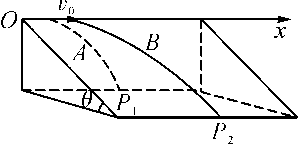
\includegraphics[width=1.35417in,height=0.65625in]{media/image170.png}\end{center}

A.A、B的运动时间相同

B.A、B沿x轴方向的位移相同

C.A、B运动过程中的加速度大小相同

D.A、B落地时速度大小相同
\begin{solution}
	设O点与水平面的高度差为h,由$h=\dfrac{1}{2} g t^{2}, \dfrac{h}{\sin \theta}=\dfrac{1}{2} g \sin \theta \cdot t_{2}^{2}$可得$t_{1}=\sqrt{\dfrac{2 h}{g}}, t_{2}=\sqrt{\dfrac{2 h}{g \sin ^{2} \theta}}$,故$t_1< t_2$,选项A错误;由$x_{1}=v_{0} t_{1}, x_{2}=v_{0} t_{2}$,可知$x_1$\textless $x_2$,选项B错误;由$a_{1}=g, a_{2}=g \sin \theta$可知,选项C错误;A落地的速度大小为$v_{A}=\sqrt{v_{0}^{2}+\left(g t_{1}\right)^{2}}=\sqrt{v_{0}^{2}+2 g h}$,B落地的速度大小$v_{B}=\sqrt{v_{0}^{2}+\left(a_{2} t_{2}\right)^{2}}=\sqrt{v_{0}^{2}+2 g h}$,所以$v_A$=$v_B$,故选项D正确.
\end{solution}

\newpage
\section{圆周运动的规律及应用}


1.描述圆周运动的物理量

\begin{longtable}[]{@{}m{2cm}m{9cm}m{4cm}@{}}
\toprule
& 定义、意义 & 公式、单位\tabularnewline
\midrule
\endhead
\begin{minipage}[t]{0.50\columnwidth}\raggedright
线速度\strut
\end{minipage} & \begin{minipage}[t]{0.60\columnwidth}\raggedright
(1)描述做圆周运动的物体运动快慢的物理量(v)

(2)是矢量,方向和半径垂直,和圆周相切\strut
\end{minipage} & \begin{minipage}[t]{0.30\columnwidth}\raggedright
(1)$v=\dfrac{\Delta s}{\Delta t}=\dfrac{2 \pi r}{T}$

(2)单位:m/s\strut
\end{minipage}\tabularnewline
\begin{minipage}[t]{0.50\columnwidth}\raggedright
角速度\strut
\end{minipage} & \begin{minipage}[t]{1\columnwidth}\raggedright
(1)描述物体绕圆心转动快慢的物理量($\omega$)

(2)中学不研究其方向\strut
\end{minipage} & \begin{minipage}[t]{0.50\columnwidth}\raggedright
(1)$\omega=\dfrac{\Delta \theta}{\Delta t}=\dfrac{2 \pi}{T}$

(2)单位:rad/s\strut
\end{minipage}\tabularnewline
\begin{minipage}[t]{0.50\columnwidth}\raggedright
周期和转速\strut
\end{minipage} & \begin{minipage}[t]{0.60\columnwidth}\raggedright
(1)周期是物体沿圆周运动一圈的时间(T)

(2)转速是物体在单位时间内转过的圈数(n),也叫频率(f)\strut
\end{minipage} & \begin{minipage}[t]{0.30\columnwidth}\raggedright
(1)$T=\dfrac{2\pi r}{v}$;单位:s

(2)n的单位r/s、r/min

(3)f的单位:Hz,$f=\dfrac{1}{T}$\strut
\end{minipage}\tabularnewline
\begin{minipage}[t]{0.50\columnwidth}\raggedright
向心加速度\strut
\end{minipage} & \begin{minipage}[t]{0.60\columnwidth}\raggedright
(1)描述速度方向变化快慢的物理量($a_n$)

(2)方向指向圆心\strut
\end{minipage} & \begin{minipage}[t]{0.30\columnwidth}\raggedright
(1)$a_{n}=\dfrac{v^{2}}{r}=\omega^{2} r$

(2)单位:$m/s^2 $\strut
\end{minipage}\tabularnewline
\begin{minipage}[t]{0.50\columnwidth}\raggedright
向心力\strut
\end{minipage} & \begin{minipage}[t]{0.60\columnwidth}\raggedright
(1)作用效果是产生向心加速度,只改变线速度的方向,不改变线速度的大小

(2)方向指向圆心\strut
\end{minipage} & \begin{minipage}[t]{0.30\columnwidth}\raggedright
(1)$F_{n}=m \omega^{2} r=m \dfrac{v^{2}}{r}=m \dfrac{4 \pi^{2}}{T^{2}} r$

(2)单位:N\strut
\end{minipage}\tabularnewline
\begin{minipage}[t]{0.50\columnwidth}\raggedright
相互关系\strut
\end{minipage} & \begin{minipage}[t]{0.60\columnwidth}\raggedright
(1)$v=r \omega=\dfrac{2 \pi r}{T}=2 \pi r f$

(2)$a_{n}=\dfrac{v^{2}}{r}=r \omega^{2}=\omega v=\dfrac{4 \pi^{2} r}{T^{2}}=4 \pi^{2} \mathrm{f}r$

(3)$F_{n}=m \dfrac{v^{2}}{r}=m r \omega^{2}=m \dfrac{4 \pi^{2} r}{I^{2}}=m \omega v=m 4 \pi^{2} R r$\strut
\end{minipage} & \begin{minipage}[t]{0.30\columnwidth}\raggedright
\strut
\end{minipage}\tabularnewline
\bottomrule
\end{longtable}

2.匀速圆周运动的向心力

(1)作用效果:产生向心加速度,只改变线速度的方向,不改变线速度的大小.

(2)大小:$F_{n}=m\dfrac{v^2}{r}=\operatorname{mr} \omega^{2}=\dfrac{{4 \pi^{2}} r}{{T}}-=m \omega v=m \cdot 4 \pi^{2} f^2 r$.

(3)方向:始终沿半径指向\_\_圆心\_\_.

(4)来源:向心力可以由一个力提供,也可以由几个力的\_\_合力\_\_提供,还可以由一个力的\_\_分力\_\_提供.

3.离心运动

(1)定义:做\_\_圆周\_\_运动的物体,在所受合力突然消失或不足以提供圆周运动所需\_\_向心力\_\_的情况下,所做的逐渐远离圆心的运动.

(2)本质:做圆周运动的物体,由于本身的惯性,总有沿着圆周切线方向飞出去的倾向.

\begin{center}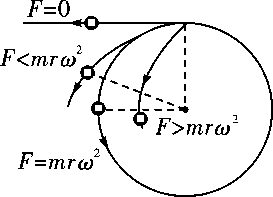
\includegraphics[width=1.23333in,height=0.9in]{media/image178.png}\end{center}

(3)受力特点

\ding{172}当$F=mω^2r$时,物体做\_\_匀速圆周\_\_运动;

\ding{173}当F=0时,物体沿\_\_切线\_\_方向飞出;

\ding{174}当$F<mω^2r$时,物体逐渐\_\_远离\_\_圆心,做离心运动.

4.近心运动

当提供向心力的合力大于做圆周运动所需向心力,即$F>mω^2r$时,物体将逐渐\_\_靠近\_\_圆心,做近心运动.

\newpage
\subsection{圆周运动中的运动学分析}

1.圆周运动各物理量间的关系

\begin{center}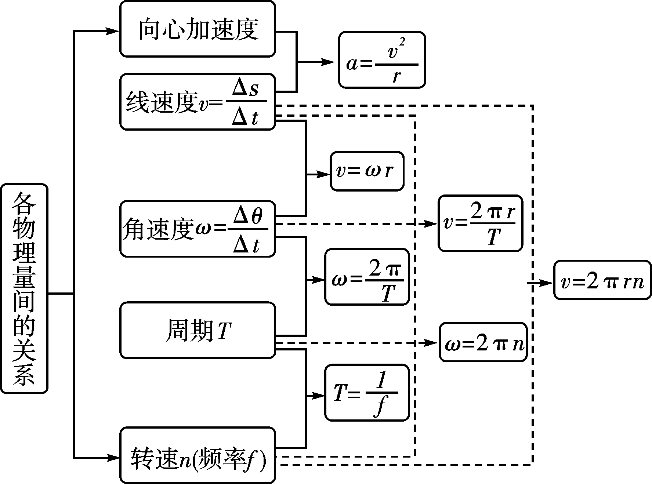
\includegraphics[width=2.96667in,height=2.2in]{media/image180.png}\end{center}

2.常见的三种传动方式及特点

(1)皮带传动:如图甲、乙所示,皮带与两轮之间无相对滑动时,两轮边缘线速度大小相等,即$v_A$=$v_B$.

\begin{center}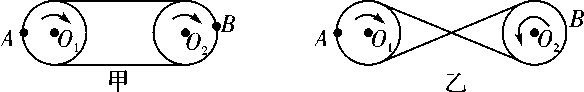
\includegraphics[width=2.65in,height=0.41667in]{media/image181.png}\end{center}

(2)摩擦传动:如图丙所示,两轮边缘接触,接触点无打滑现象时,两轮边缘线速度大小相等,即$v_A$=$v_B$.

\begin{center}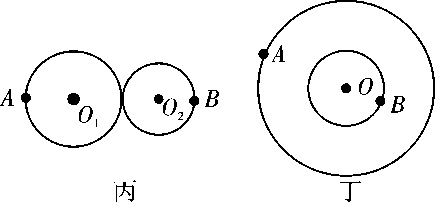
\includegraphics[width=1.98333in,height=0.91667in]{media/image182.png}\end{center}

(3)同轴传动:如图丁所示,两轮固定在一起绕同一转轴转动,两轮转动的角速度大小相等,即$\omega_A=\omega_B$.

\begin{center}
\includegraphics[width=0.71667in,height=0.13333in]{media/image37.png}

\textbf{解答传动装置类问题的方法}
\end{center}


(1)确定所研究问题属于哪类传动方式,抓住传动装置的特点.

\ding{172}同轴传动:固定在一起共轴转动的物体上各点角速度相同;\ding{173}皮带传动、齿轮传动和摩擦传动:皮带(或齿轮)传动和不打滑的摩擦传动的两轮边缘上各点线速度大小相等.

(2)结合公式v=$\omega$r,v一定时$\omega$与r成反比,$\omega$一定时v与r成正比,判定各点v、$\omega$的比例关系,若判定向心加速度a的比例,巧用a=$\omega$v这一规律.



\newpage
\subsection{圆周运动中的动力学分析}

\begin{center}
\includegraphics[width=0.71667in,height=0.13333in]{media/image13.png}

\textbf{解答圆周运动中的动力学问题的分析思路}
\end{center}


(1)几何关系的分析,目的是确定圆周运动的圆心、半径等.

(2)运动分析,目的是表示出物体做圆周运动所需要的向心力.

(3)受力分析,目的是利用力的合成与分解知识,表示出物体做圆周运动时,外界所提供的向心力.

{[}例2{]}(2018·湖北武汉模拟)(多选)如图甲所示,一根细线上端固定在S点,下端连一小铁球A,让小铁球在水平面内做匀速圆周运动,此装置构成一圆锥摆(不计空气阻力).下列说法中正确的是( AC )

\begin{center}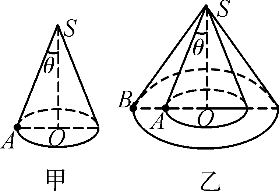
\includegraphics[width=1.26667in,height=0.86667in]{media/image184.png}\end{center}

A.小球做匀速圆周运动时的角速度一定大于$\sqrt{\dfrac{g}{l}}$(l为摆长)

B.小球做匀速圆周运动时,受到重力、细线的拉力和向心力作用

C.另有一个圆锥摆,摆长更大一点,两者悬点相同,如图乙所示,如果改变两小球的角速度,使两者恰好在同一水平面内做匀速圆周运动,则B球的角速度等于A球的角速度

D.如果两个小球的质量相等,则在图乙中两根细线受到的拉力相等
\begin{solution}
	小球受力如图所示,由圆周运动规律可得$F_{\mathrm{n}}=m r \omega^{2}, \quad$ 又 $F_{\mathrm{n}}=m g \tan \theta,$ 解得 $\omega=\sqrt{\dfrac{\operatorname{gtan} \theta}{r}}, r=l \sin \theta$,可得$\omega=\sqrt{\dfrac{g}{l \cos \theta}}\left(0^{\circ}<\theta<90^{\circ}\right)$,可知小球做匀速圆周运动时的角速度一定大于$\sqrt{\dfrac{g}{l}}$,故选项A正确;向心力是效果力,匀速圆周运动的向心力是由合力提供的,小球做匀速圆周运动时,重力和细线的拉力的合力充当向心力,故选项B错误;由$\omega=\sqrt{\dfrac{g}{l \cos \theta}}$,$\operatorname{lcos} \theta=h$,所以$\omega$=$\sqrt{\dfrac{g}{l}}$,由于高度相同,B球的角速度等于A球的角速度,故选项C正确;由图可知$T=\dfrac{m g}{\cos \theta}$,由于$\theta_{B}>\theta_{A}$,如果两个小球的质量相等,则$T_{B}>T_{A}$,故选项D错误.
\end{solution}

\begin{center}
\includegraphics[width=0.71667in,height=0.13333in]{media/image25.png}

\textbf{圆周运动中的动力学分析思路}
\end{center}
确定研
究对象 $\rightarrow$ 对其受
力分析 $\rightarrow$ 确定轨
迹平面 $\rightarrow$ 找出向
心力 $\rightarrow$ 由牛顿第二定律
确定各量关系

\newpage
\subsection{水平转盘中圆周运动物体的临界问题}

1.判断临界状态:有些题目中有``刚好''\,``恰好''\,``正好''等字眼,明显表明题述的过程存在着临界点;若题目中有``取值范围''\,``多长时间''\,``多大距离''等词语,表明题述的过程存在着``起止点'',而这些起止点往往就是临界状态;若题目中有``最大''\,``最小''\,``至多''\,``至少''等字眼,表明题述的过程存在着极值,这个极值点也往往是临界状态。

2.确定临界条件:判断题述的过程存在临界状态之后,要通过分析弄清临界状态出现的条件,并以数学形式表达出来.

3.选择物理规律:当确定了物体运动的临界状态和临界条件后,对于不同的运动过程或现象,要分别选择相对应的物理规律.然后再列方程求解.

{[}例3{]}(2018·江苏苏州调研)如图所示,用一根长为l=1m的细线,一端系一质量为m=1kg的小球(可视为质点),另一端固定在一光滑锥体顶端,锥面与竖直方向的夹角$\theta=37^\circ$,当小球在水平面内绕锥体的轴做匀速圆周运动的角速度为$\omega$时,细线的张力为$F_T$.求:($\sin=0.6$,$\cos37^\circ=0.8$,g取 $10m/s^2$,结果可用根式表示)

(1)若要小球刚好离开锥面,则小球的角速度$\omega_0$至少为多大?

(2)若细线与竖直方向的夹角为$60^\circ$,则小球的角速度$\omega^{'}$为多大?

\begin{center}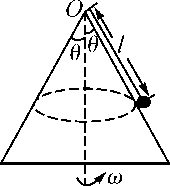
\includegraphics[width=0.76667in,height=0.85in]{media/image185.png}\end{center}


\begin{solution}(1) $\dfrac{5}{2} \sqrt{2} \mathrm{rad} / \mathrm{s}$ (2)$2 \sqrt{5} \mathrm{rad} / \mathrm{s}$

	(1)若要小球刚好离开锥面,则小球只受到重力和细线的拉力,受力分析如图所示.小球做匀速圆周运动的轨迹圆在水平面上,故向心力水平,在水平方向运动用牛顿第二定律及向心力公式得

\begin{center}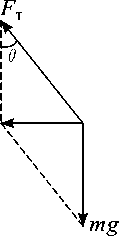
\includegraphics[width=0.55in,height=1.06667in]{media/image186.png}\end{center}

$m g \tan \theta=m \omega_{0}^{2} l \sin \theta$

解得 $\omega_{0}^{2}=\dfrac{g}{l \cos \theta}$

即 $\omega_{0}=\sqrt{\dfrac{g}{l \cos \theta}}=\dfrac{5}{2} \sqrt{2} \mathrm{rad} / \mathrm{s}$

(2)同理,当细线与竖直方向成$60^\circ$角时,由牛顿第二定律及向心力公式得

$mg\tan \alpha=m \omega^{\prime} \operatorname{lsin} \alpha$

解得 $\omega^{\prime 2}=\dfrac{g}{l \cos \alpha},$ 即

$\omega^{\prime}=\sqrt{\dfrac{g}{l \cos \alpha}}=2 \sqrt{5} \mathrm{rad} / \mathrm{s}$
\end{solution}
\newpage
\subsection{竖直面内圆周运动物体的临界问题}

在竖直平面内做圆周运动的物体,按运动到轨道最高点时的受力情况可分为两类:一是无支撑(如球与绳连接、沿内轨道运动的过山车等),称为``绳(环)约束模型'',二是有支撑(如球与杆连接、在弯管内的运动等),称为``杆(管)约束模型''.下面对绳、杆模型涉及的临界问题进行比较,分析如下:

\begin{longtable}[]{@{}m{1.5cm}m{6cm}m{6cm}@{}}
\toprule

&
轻绳牵球
&
轻杆牵球
\tabularnewline
\midrule
\endhead
图例 &
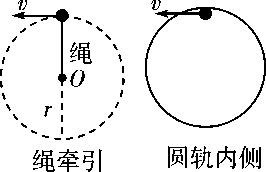
\includegraphics[width=1.21667in,height=0.78333in]{media/image187.png} 
&
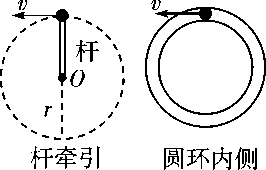
\includegraphics[width=1.21667in,height=0.76667in]{media/image188.png}
\tabularnewline
实例 
& 
球绳连接、水流星、沿内轨道过山车等 
&
球杆连接、过拱桥等(注意过拱桥与球杆连接的区别)
\tabularnewline
受力

示意图 
&
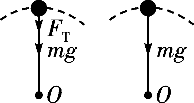
\includegraphics[width=0.88333in,height=0.46667in]{media/image189.png} 
&
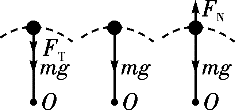
\includegraphics[width=1.06667in,height=0.5in]{media/image190.png}
\tabularnewline
最高点

临界条件 
&
根据$mg=\dfrac{mv_{\text{临界}}^2}{r}$,则$v_{\text{临界}}=\sqrt{gr}$
&
由于杆的支撑作用,$v_{\text{临界}}=0$
\tabularnewline
最高点

受力

与

运动情况
讨论分析
&

\ding{172}能过最高点的条件$v\geq v_{\text{临界}}=\sqrt{gr}$

$F_T+mg=m\dfrac{v^2}{r} $,绳、轨道对球产生弹力$F_T\geq 0$,方向指向圆心;

\ding{173}不能过最高点的条件$v< v_{\text{临界}}=\sqrt{gr}$,在到达最高点前小球已经脱离了圆周轨道
&
\ding{172}当v=0时,杆对小球有竖直向上的支持力$F_N$,且$F_N=mg$; 

\ding{173}当$0<v<\sqrt{g r}$时,杆对小球有竖直向上的支持力$F_N$,其大小随速度的增大而减小,且$0<F_{\mathrm{N}}<m g$;

\ding{174}当$v=\sqrt{g r}$时,杆对小球没有作用力,即$F_T=0$;

\ding{175}当$v>\sqrt{g r}$时,杆对小球有竖直向下的拉力$F_N$,其大小随速度的增大而增大
\tabularnewline
\bottomrule
\end{longtable}

\begin{center}
\includegraphics[width=0.71667in,height=0.13333in]{media/image13.png}

\textbf{竖直面内圆周运动类问题的解题技巧}
\end{center}


(1)定模型:首先判断是轻绳模型还是轻杆模型,两种模型过最高点的临界条件不同.

(2)确定临界点:抓住绳模型中最高点$v \geq \sqrt{g r}$及杆模型中$v \geq 0$这两个临界条件.

(3)研究状态:通常情况下竖直平面内的圆周运动只涉及最高点和最低点的运动情况.

(4)受力分析:对物体在最高点或最低点时进行受力分析,根据牛顿第二定律列出方程,$F_{\text {合 }}=F_{\text {向 }}$.

(5)过程分析:应用动能定理或机械能守恒定律将初、末两个状态联系起来列方程.

\newpage
\section{万有引力与航天}


1.开普勒三定律的内容、公式

\begin{longtable}[]{@{}m{3cm}m{6.5cm}m{3.5cm}@{}}
\toprule
定律 & 内容 & 图示或公式\tabularnewline
\midrule
\endhead
开普勒第一定律(轨道定律) &所有行星绕太阳运动的轨道都是椭圆,太阳处在椭圆的一个焦点上&
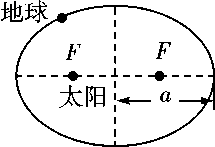
\includegraphics[width=0.98333in,height=0.66667in]{media/image198.png}\tabularnewline
开普勒第二定律(面积定律) &对任意一个行星来说,它与太阳的连线在相等的时间内扫过的面积相等 &
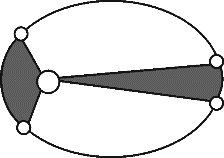
\includegraphics[width=1.01667in,height=0.71667in]{media/image199.png}\tabularnewline
开普勒第三定律(周期定律)&所有行星的轨道的半长轴的三次方跟它的公转周期的二次方的比值都相等& 
$\dfrac{a^{3}}{T^{2}}=k$, $k$是一个与行星无关的常量\tabularnewline
\bottomrule
\end{longtable}

2.万有引力定律

(1)内容:自然界中任何两个物体都是相互吸引的,引力的大小与\_\_两物体的质量的乘积\_\_成正比,与\_\_两物体间的距离的二次方\_\_成反比.

(2)公式:$F=G\dfrac{m_1m_2}{r^2}$,其中G为万有引力常量,$G=6.67\times 10^{-11} N·m^2/kg^2$,其值由卡文迪许通过扭秤实验测得.

(3)使用条件:适用于两个\_\_质点\_\_或均匀球体;r为两质点或均匀球体球心间的距离.

3.宇宙速度

(1)第一宇宙速度

\ding{172}第一宇宙速度又叫\_\_环绕\_\_速度,其数值为\_\_7.9\_\_km/s.

\ding{173}第一宇宙速度是人造卫星在\_\_地面\_\_附近环绕地球做匀速圆周运动时具有的速度.

\ding{174}第一宇宙速度是人造卫星的最小\_\_发射\_\_速度,也是人造卫星的最大\_\_环绕\_\_速度.

\ding{175}第一宇宙速度的计算方法.

由 $G \dfrac{M m}{R^{2}}=m \dfrac{\nu^{2}}{R}$ 得 $v=\sqrt{\dfrac{G M}{R}}$;

由 $m g=m_{R}^{\nu}$ 得 $v=\sqrt{g R}$.

(2)第二宇宙速度

使物体挣脱\_\_地球\_\_引力束缚的最小发射速度,其数值为\_\_11.2\_\_km/s.

(3)第三宇宙速度

使物体挣脱\_\_太阳\_\_引力束缚的最小发射速度,其数值为\_\_16.7\_\_km/s.

\newpage
\subsection{万有引力定律的理解与应用}

1.地球表面的重力与万有引力

地面上的物体所受地球的吸引力产生两个效果,其中一个分力提供了物体绕地轴做圆周运动的向心力,另一个分力等于重力.

(1)在两极,向心力等于零,重力等于万有引力;

(2)除两极外,物体的重力都比万有引力小;

(3)在赤道处,物体的万有引力分解为两个分力$F_{\text {向 }}$和mg刚好在一条直线上,则有$F=F_{\text {向 }}+m g,$ 所以 $m g=F-F_{\text {向 }}=\dfrac{G M m}{R^{2}}-m R \omega_{\text {自 }}^{2}$.

2.地球表面附近(脱离地面)的重力与万有引力

物体在地球表面附近(脱离地面)时,物体所受的重力等于地球表面处的万有引力,即$m g=\dfrac{G M m}{R^{2}}$,R为地球半径,g为地球表面附近的重力加速度,此处也有$G M=g R^{2}$.

3.距地面一定高度处的重力与万有引力

物体在距地面一定高度h处时,$m g^{\prime}=\dfrac{G M m}{(R+h)^{2}}$,R为地球半径,$g^{'}$为该高度处的重力加速度.



\subsection{天体的质量和密度的计算}

1.``g、R''计算法

利用天体表面的重力加速度g和天体半径R

(1)由$G \dfrac{M m}{R^{2}}=m g$ 得天体质量 $M=\dfrac{g R^{2}}{G}$.

(2)天体密度$\rho=\dfrac{M}{V}=\dfrac{M}{\dfrac{4}{3} \pi R^{3}}=\dfrac{3 g}{4 \pi G R}$.

2.``T、r''计算法

测出卫星绕天体做匀速圆周运动的半径r和周期T

(1)由$G \dfrac{M m}{r^{2}}=m \dfrac{4 \pi^{2} r}{T^{2}}$ 得天体的质量 $M=\dfrac{4 \pi^{2} r^{3}}{G T^{2}}$.

(2)若已知天体的半径R,则天体的密度$\rho=\dfrac{M}{V}=\dfrac{M}{\dfrac{4}{3} \pi R^{3}}=\dfrac{3 \pi r^{3}}{G T^{2} R^{3}}$. 

(3)若卫星绕天体表面运行时,可认为轨道半径r等于天体半径R,则天体密度$\rho=\dfrac{3 \pi}{G T^{2}}$,可见,只要测出卫星环绕天体表面运动的周期T,就可估算出中心天体的密度.


\begin{center}
\includegraphics[width=0.71667in,height=0.13333in]{media/image34.png}

\textbf{估算天体质量和密度时应注意的问题}
\end{center}


(1)利用万有引力提供天体做圆周运动的向心力估算天体质量时,估算的只是中心天体的质量,并非环绕天体的质量.

(2)区别天体半径R和卫星轨道半径r,只有在天体表面附近的卫星才有$r\approx ≈R$;计算天体密度时,$V=\dfrac{4}{3} \pi R^{3}$中的R只能是中心天体的半径.

\newpage
\subsection{人造卫星的运行规律}

1.卫星的各物理量随轨道半径变化的规律

高轨低速大周期

\begin{center}
\includegraphics[width=0.71667in,height=0.13333in]{media/image44.png}\end{center}

(1)解决力与运动关系的思想还是动力学思想,解决力与运动的关系的桥梁还是牛顿第二定律.

(2)卫星的$a_n$、v、$\omega$、T是相互联系的,其中一个量发生变化,其他各量也随之发生变化.

(3)$a_n$、v、$\omega$、T均与卫星的质量无关,只由轨道半径r和中心天体质量共同决定.

\begin{center}
\includegraphics[width=0.71667in,height=0.13333in]{media/image34.png}

\textbf{同步卫星的六个``一定''}
\end{center}


\begin{center}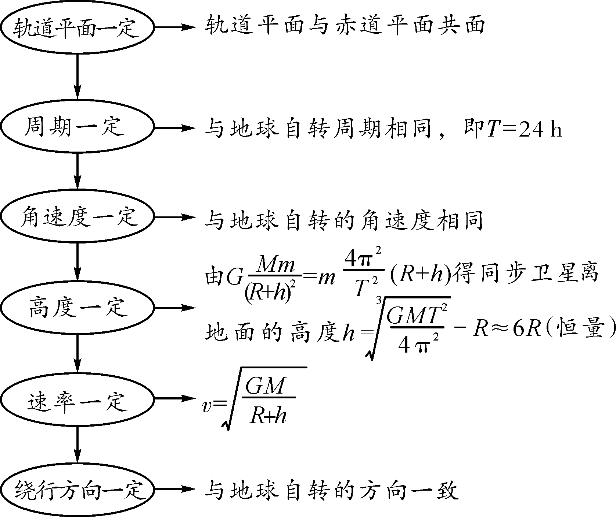
\includegraphics[width=2.8in,height=2.35in]{media/image201.png}\end{center}
\newpage
\subsection{卫星(航天器)的变轨问题及对接问题}

\begin{center}
\includegraphics[width=0.71667in,height=0.13333in]{media/image37.png}\end{center}

(1)航天器变轨问题的三点注意

\ding{172}航天器变轨后稳定在新轨道上的运行速度由$v=\sqrt{\dfrac{G M}{r}}$判断.

\ding{173}航天器在不同轨道上运行时机械能不同,轨道半径越大,机械能越大.

\ding{174}航天器经过不同轨道相交的同一点时加速度相等,外轨道的速度大于内轨道的速度.

(2)变轨的两种情况
较低圆轨道$\xLongleftrightarrow[\text{近地点向前喷气}]{\text{近地点向后喷气}} $ 椭圆轨道$\xLongleftrightarrow[\text{远地点向前喷气}]{\text{远地点向后喷气}} $较高圆轨道
\subsection{天体运动中的``多星''系统}

 在天体运动中,离其他星体较远的几颗星,在它们相互间万有引力的作用力下绕同一中心位置运转,这样的几颗星组成的系统称为宇宙多星模型.

1.``双星''系统

(1)两颗恒星做匀速圆周运动所需的向心力是由它们之间的万有引力提供的,故两恒星做匀速圆周运动的向心力大小相等.

(2)两颗恒星均绕它们连线上的一点做匀速圆周运动,因此它们的运行周期和角速度是相等的.

(3)两颗恒星做匀速圆周运动的半径$r_1$和$r_2$与两行星间距L的大小关系$r_1+r_2=L$.

2.``多星''系统

(1)多颗行星在同一轨道绕同一点做匀速圆周运动,每颗行星做匀速圆周运动所需的向心力由其他各个行星对该行星的万有引力的合力提供.

(2)每颗行星转动的方向相同,运行周期、角速度和线速度大小相等.



\begin{center}\includegraphics[width=0.71667in,height=0.13333in]{media/image13.png}

\textbf{天体运动中的``多星''系统特点}
\end{center}


(1)不论是双星还是三星系统模型,每个星体都做匀速圆周运动(中心星体除外),且周期、角速度相等.

(2)注意应用数学知识,由星体距离求轨道半径.

(3)只有当系统中星体质量相等时,它们的轨道半径才相等.
\newpage
\begin{problemset}
	\item 引力势能
	\begin{itemize}
		\item 定义:物体(特别指天体)在引力场中具有的势能叫做引力势能,引力势能是标量,单位为焦(J)。重力势能是引力势能在特殊情况下的表达形式。
		\item 公式:$E_p=-\dfrac{GMm}{r}$
		\item 数学推导
		质量为m的物体轨道半径为r,则引力势能应该等于物体移动到零势能面引力做的功
		
		$\begin{aligned} 
		E_p &=W_{\text{引}} \\
		 &=F_{\text{万}}x\\
		  &=-\int_r^{\infty}G\dfrac{Mm}{x^2}· dx\\
		  &=-GMm[-x]_r^{+\infty}\\
		  &=-GMm\times 0+GMm\times r^{-1}\\
		  &=-\dfrac{GMm}{r}
		 \end{aligned}$
	\end{itemize}
\end{problemset}
